\section{Visualizing taxonomies and connectivity data}
\label{sect:visualization}

Treemaps~\cite{JS91} are an effective technique to visualize hierarchical data by using nested shapes in a space-filling layout.
Each shape represents a geometric region, which can be subdivided recursively into smaller regions. The standard shape is the rectangle.
Nodes in a treemap, also called \emph{tiles}, represent individual data items in a dataset. Node size, color and text label can be used to represent attributes of the data item. One-layered treemaps can display data attributes but are not very good at emphasizing the place of an item in the overall hierarchical structure. To compensate for that, a small margin with structural labels is typically used. In treemaps displaying hierarchical structures, it is possible to navigate among different layers and zoom into selected tiles~\cite{BL07}.

To create a treemap, one must define a tiling algorithm - a way to divide a tile into sub-tiles of specified areas.
Tiling algorithms used for typical applications of treemaps such as e.g., visualization of folders in files in the computer file system with their respected sizes, do not associate tile positions with any characteristic of the data. This is not the case in our scenario: while a user navigates among different layers, filters data and zooms into selected areas, the tool should keep the tiles associated with the data in the same relative positions to each other. Otherwise, the user's perception of the displayed information will be quickly affected. Moreover, our tiling algorithm should allow the user to enforce constraints on tile positions to make the treemap views structurally resemble body regions. Hence, we developed a stable and customizable tiling algorithm that arranges tiles corresponding to data items according to a given template~\cite{KBK14}.

For a set of $n$ data items with no positional constraints, a default template is created that consists of $\lfloor \sqrt{n} \rfloor$ rows and $\lceil sqrt(n) \rceil$ columns in each row but the last one (which may contain less columns). If the positional data is available (e.g., FMA ontology adjacent-to relation) or a user wants to rearrange the data manually, a custom template is associated with the parent node of the dataset items. The template is a hierarchical structure
$\{splitType, \{\},..., \{\}\}$ where $splitType \in \{slice, dice\}$ defines a way to split the rectangle into sub-rectangles: vertically or horizontally. By recursively splitting the available area into sub-rectangles, one can define complex layouts that enforce two dimensional constraints in the form ``\emph{x} is left/right of \emph{y}'' or ``\emph{x} is above/below of \emph{y}'' where $x$ and $y$ are individual data items or groups of data items that in their turn can be allocated as needed using the same technique.

%Example here: default template + rearranged items (left -//- vs right -//-).
\subsection{Connectivity data}

We use treemap-based body plans as background to overlay the schematic representation of biological systems such as
circulatory, respiratory, or nervous systems. Body systems are essentially graphs or hypergraphs with nodes corresponding to body parts (treemap tiles), entities that belong to body parts (proteins, cells, etc.) or auxiliary nodes that are not displayed on the treemap but still carry important biomedical information, while their edges or paths represent organ system compounds such as blood vessels or nervous connections that pass through the certain body parts or its sub-parts.

Body systems are intrinsically complex and require efficient data visualization techniques that would help us to avoid clutters induced by the large amount of graph edges and their crossings and allow users to overview large parts of the body systems as well as to trace individual connections and analyze their structure. Edge bundling techniques have been proposed to improve perception of connectivity data in large dense graphs.
Such techniques generally rely on edge rerouting strategies that are either solely target at improving visual perception of edges constrained by positions of nodes or exploit the relations among connectivity data as guidelines for more natural allocation of graph edges and nodes. Our application requires the mixture of these techniques

As example, we consider the schematic visualization of blood vessels in human body.
The initial dataset is a graph extracted from the FMA database which consists of approximately 11,300 edges and over 10,000 distinct nodes.
An edge represents an unbranched segment of a blood vessel. Nodes represent junctions between blood vessel segments.
Samples of records from the dataset are shown in Table~\ref{tab:vascular-connectivity}. The first column in the dataset is a unique vascular segment identifier (ID). The second column bears the vessel type, i.e. any one of four numbers that give an indication of the biological type of segment:
1 - for arterial segment, 2 - microcirculation (MC), there are three types of MC edges: arteriole, capillary and venule, 3 - venous, and 4 - cardiac chamber.
The third column bears FMA IDs. For non-MC edges (i.e. vessels of type 1, 3 or 4) the number in this column is the FMA ID of the blood vessel of
which that segment is part (e.g. there are over 50 segments/edges that form part of the trunk of the aorta, i.e., FMA ID 50010931). For MC edges (type 2), the FMA ID is that of the body region in which the MC is embedded. The fourth and fifth columns in the dataset bear the unique node identifiers in an edge pair.
The sixth column is a free-text label describing that segment (i.e. edge).

\begin{table}
\caption{Vascular connectivity data from the FMA ontology}
\begin{tabular}{|l|l|l|l|l|p{7cm}|}
  \hline
  Segment & Type & FMA & Node 1 & Node 2 & Description \\
  \hline
  121a & 2 & 62528 & 62528\_2 & 62528\_4 & Arterioles in Microcirculation segment of Wall of left inferior lobar bronchus \\
  121c & 2 & 62528 & 62528\_4 & 62528\_5 & Capillaries in Microcirculation segment of Wall of left inferior lobar bronchus\\
  121v & 2 & 62528 & 62528\_3 & 62528\_5 & Venules in Microcirculation segment of Wall of left inferior lobar bronchus\\
  ... &... & ...   & ...      & ...      & ...\\
  8499 & 1 & 69333 & 8498\_0 & 62528\_2  & Arterial Segment 8499 of Trunk
of left second bronchial artery from origin of supplying terminal segment
to the arteriolar side of the Wall of left inferior lobar bronchus
MC\\
  9547 & 3 & 66699 & 9546\_0 & 62528\_3 & Venous Segment 9547 of Trunk of
left bronchial vein from origin of supplying terminal segment to the
venular side of the Wall of left inferior lobar bronchus MC \\
  \hline
\end{tabular}
\label{tab:vascular-connectivity}
\end{table}

When it comes to describing routes of blood passage through the heart, one has to distinguish between cardiac chambers, (i.e. main lumen of left ventricle, left atrium, right ventricle or right atrium) and the MC of the wall of heart (e.g. wall of left ventricle (FMA ID 7101), left atrium (7097), right ventricle (7098) or right atrium (7096)). There are two ways by which blood passes through the heart: (i) though the chambers and (ii) through its walls. Consequently, we exclude cardiac chamber segments from consideration as they are redundant for the representation of vascular connectivity data in our application.
An MC is represented by three edges connected in series: one edge represents tissue arterioles, a second edge stands for the bed of
capillaries, while a third denotes the venules. In one MC, therefore: a) the end node of the arteriolar edge and the start node of the
capillary edge are equivalent, and b) the end node of the capillary edge and the end node of the venular
edge are equivalent.

In the above example, the anatomical entity in which the MC is embedded is 62528 - the topology of MC segment connectivity is as follows:
$$62528\_2 - [121a] \rightarrow 62528\_4 - [121c] \rightarrow 62528\_5 \leftarrow [121v] - 62528\_3.$$
MC segment 121a is supplied with blood by the arterial segment 8499 while MC segment 121v is drained of blood by the venous segment 9547.

The accurate visualization of the cardiovascular system in a comprehensible way requires complex pre-processing (about 12 rules were identified to extract the data of interest from the presented dataset by a biomedical expert in our team).
In this paper, for the illustration purpose we show only paths connecting MCs of the walls of the heart to MCs belonging to the sub-organs of the organs in our 24 upper level tile body plan.
To obtain this view, we looked for the shortest paths (due to the way the data is represented in the initial data set, loops are possible) from the MCs of the heart walls to the final FMA tiles. For example, the path from the left ventricle to the wall of left inferior lobar bronchus MC is as follows:
$7101 \rightarrow 2406 \rightarrow 2407 \rightarrow 2573 \rightarrow 2657 \rightarrow 3780 \rightarrow 4288 \rightarrow 4707 \rightarrow 4709 \rightarrow 4711 \rightarrow 4713 \rightarrow 4714 \rightarrow 8492 \rightarrow 8494 \rightarrow 8496 \rightarrow 8498 \rightarrow 8499 \rightarrow 62528,$
while the path from this organ to the right atrium is
$7096 \leftarrow 771 \leftarrow 1333 \leftarrow 1334 \leftarrow 1731 \leftarrow 1993 \leftarrow 1994 \leftarrow 1996 \leftarrow 1998 \leftarrow 1999 \leftarrow 1983 \leftarrow 9534 \leftarrow 9536 \leftarrow 9538 \leftarrow 9540 \leftarrow 9542 \leftarrow 9544 \leftarrow 9546 \leftarrow 9547 \leftarrow 62528.$

The first and the last IDs in this path correspond to the tiles in the treemap view, while the intermediate IDs will be represented using auxiliary nodes with undefined coordinates. One of the issues we encountered is the need to determine optimal positions for these nodes. Since several paths as above can have common sub-paths, the intermediate nodes should not deviate too much from the way from the heart MC to each of the end tiles sharing such sub-paths. This motivates our application of the sticky force-directed graph visualization method that given a sub-set of nodes with fixed coordinates arrange other nodes to optimize forces on the graph edges. As our only objective is to allocate intermediate nodes as close to the paths they belong to (which most naturally can be represented by straight lines) as possible, we set gravity and charge to 0 and the desired link length to a minimal possible length. The extracted connectivity graphs for two heart walls: left ventricle (7101) and right atrium (7096), are shown in Figures~\ref{fig:force-7101} and \ref{fig:force-7096}.

Once the coordinates for all connectivity graph nodes are determined, we apply hierarchical edge bundling method that uses the path structure to bundle paths with common sub-paths in the graph obtained on the first stage. The final set of paths from left ventricle and right atrium are shown in Figures~\ref{fig:bundled-7101} and \ref{fig:bundled-7096}, respectively. In these images, both left ventricle and right atrium are descendants of tile 6000009: Vascular Cardiac. By setting bundling algorithm tension parameter close to 1 (0.96-0.99), we obtain a view that clearly shows that individual paths extracted from our dataset form ``highways'' which correspond to major arteries and veins in the human body.

\begin{figure*}
\centering
  \subfigure[Arterial connections from left ventricle]{
    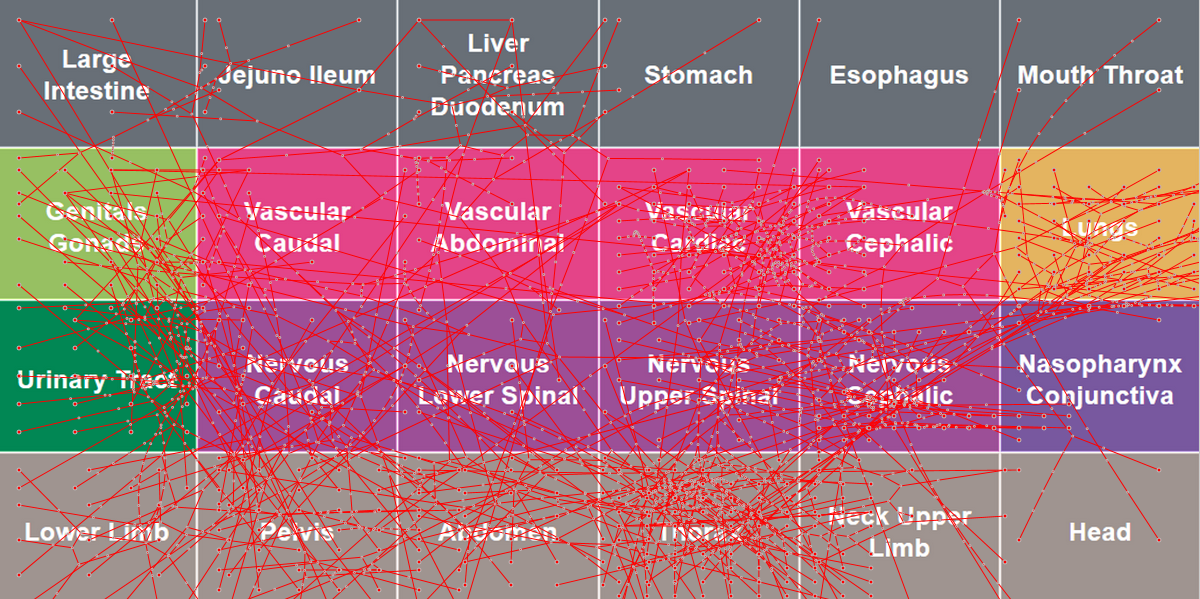
\includegraphics[width=5.8cm]{images/force-7101.png}
    \label{fig:force-7101}
  }
  \subfigure[Venous connections to right atrium]{
    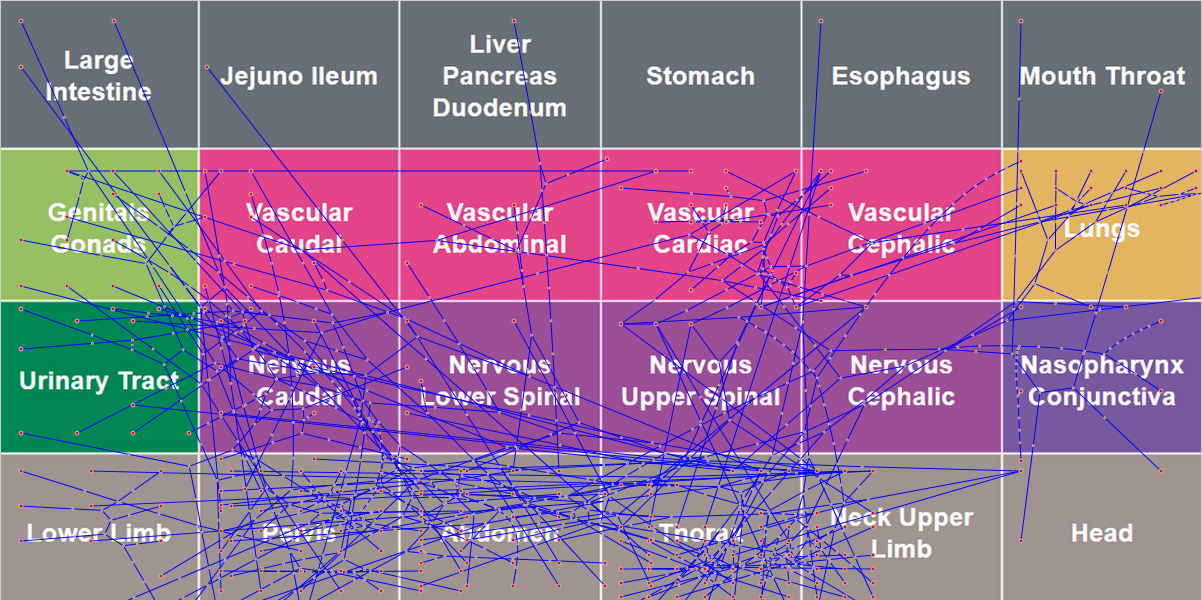
\includegraphics[width=5.8cm]{images/force-7096b.png}
    \label{fig:force-7096}
  }
  \subfigure[Bundled paths from left ventricle]{
    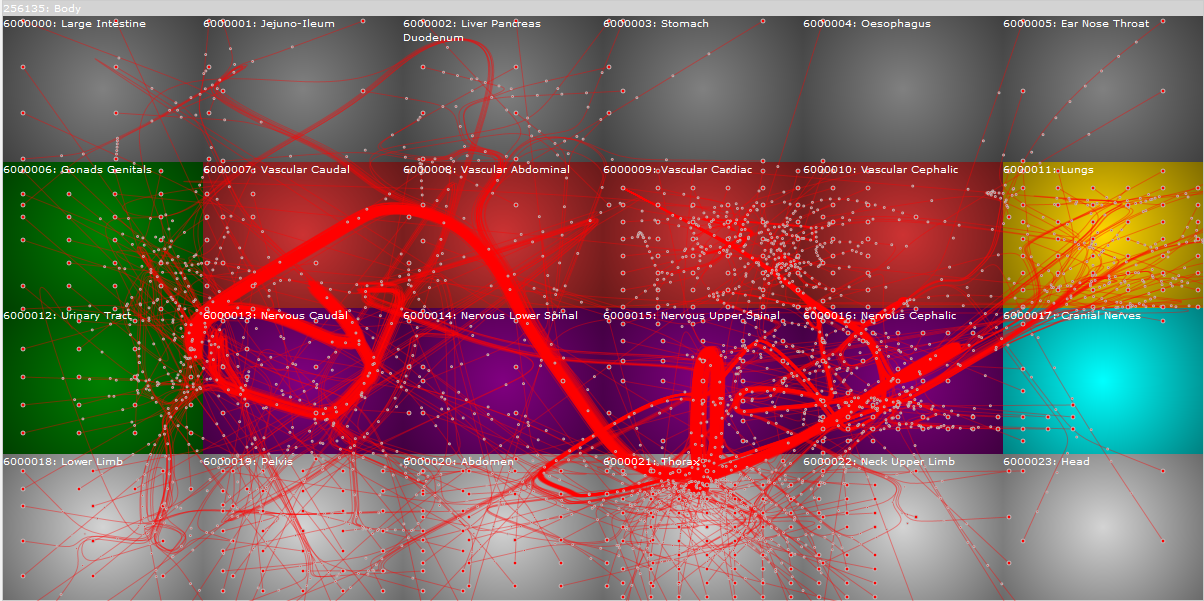
\includegraphics[width=5.8cm]{images/connections-7101.png}
    \label{fig:bundled-7101}
  }
  \subfigure[Bundled paths to right atrium]{
    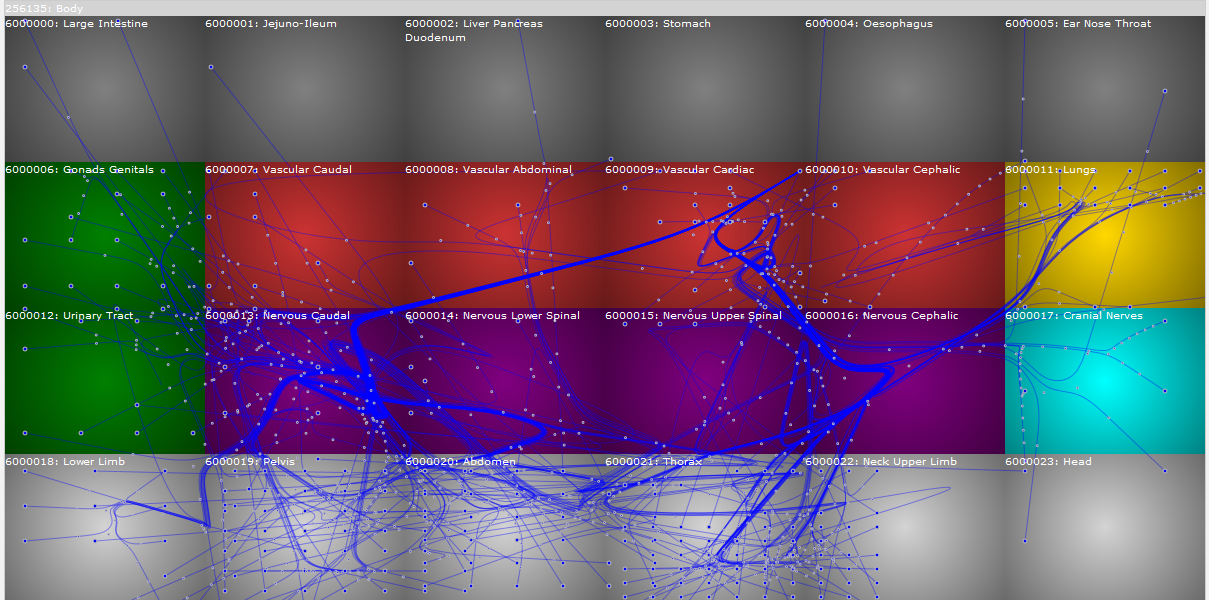
\includegraphics[width=5.8cm]{images/connections-7096b.png}
    \label{fig:bundled-7096}
  }
  \caption{Cardiovascular system}
  \label{fig:vascular-connectivity}
\end{figure*}

After one-time pre-processing to import data from available external sources, we store connectivity data in a generic JSON format. A user can interact with and edit these data using functionality of our application. One of the prime goals of our tools is to simplify the access and maintenance of biomedical taxonomies, vascular system among others. A user should be able to choose a way to represent connectivity data. There is ongoing work on the implementation of the orthogonal connector visualization algorithm that would place links into margins between tiles so that they will not obstruct the interaction with the tiles.


